\documentclass[10pt]{article}
\usepackage[margin=.8in]{geometry}\usepackage{graphicx,booktabs,xcolor,microtype,parskip}
\definecolor{navy}{HTML}{18334B}\definecolor{teal}{HTML}{176B87}
\usepackage[colorlinks=true,linkcolor=teal,urlcolor=teal]{hyperref}
\title{\vspace{-2em}\color{navy}\bfseries IDM-Viz cluster localization sensitivity\\[-.2em]\large Frozen representations and many-to-one historical mappings}
\author{Post-deadline empirical addendum}\date{17 November 2026}
\begin{document}\maketitle\vspace{-1.1em}
\section*{Protocol}
We tested 30 already locked evaluation seeds, five generating regions, and 3, 5, or 10 clusters. Cluster models, standardization, and PCA bases were fit on historical training features only. Region mappings and per-cluster region probabilities were estimated from those same historical rows. Monitoring region IDs were used only for scoring. We compare scaled full-feature clustering with frozen PCA-2 and PCA-3 clustering. The many-to-one mapping permits several clusters to represent one region; Jeffreys-style additive smoothing (0.5 per cell) defines the cluster-to-region probabilities. Intervals resample seeds (5000{} replicates), not rows. This is an exploratory diagnostic on the locked seed bank; the primary detector and original results are unchanged.
\section*{Findings}
At five clusters, full-space many-to-one macro F1 was 0.300{} (95\% seed-bootstrap CI 0.281{}--0.320{}); PCA-2 was 0.307{} and PCA-3 was 0.290{}. Five-cluster adjusted Rand index in the full space was 0.087{} (CI 0.078{}--0.096{}). Region-2 average precision was 0.213{} (CI 0.210{}--0.215{}). Allowing many-to-one maps avoids the artificial unmapped-cluster penalty, but it does not make region identities recoverable: region-2 precision/recall and ranking remain weak. PCA does not improve the five-cluster macro F1 in this experiment. These results support exposing cluster ambiguity and composition rather than presenting clusters as known generating regions.
\begin{center}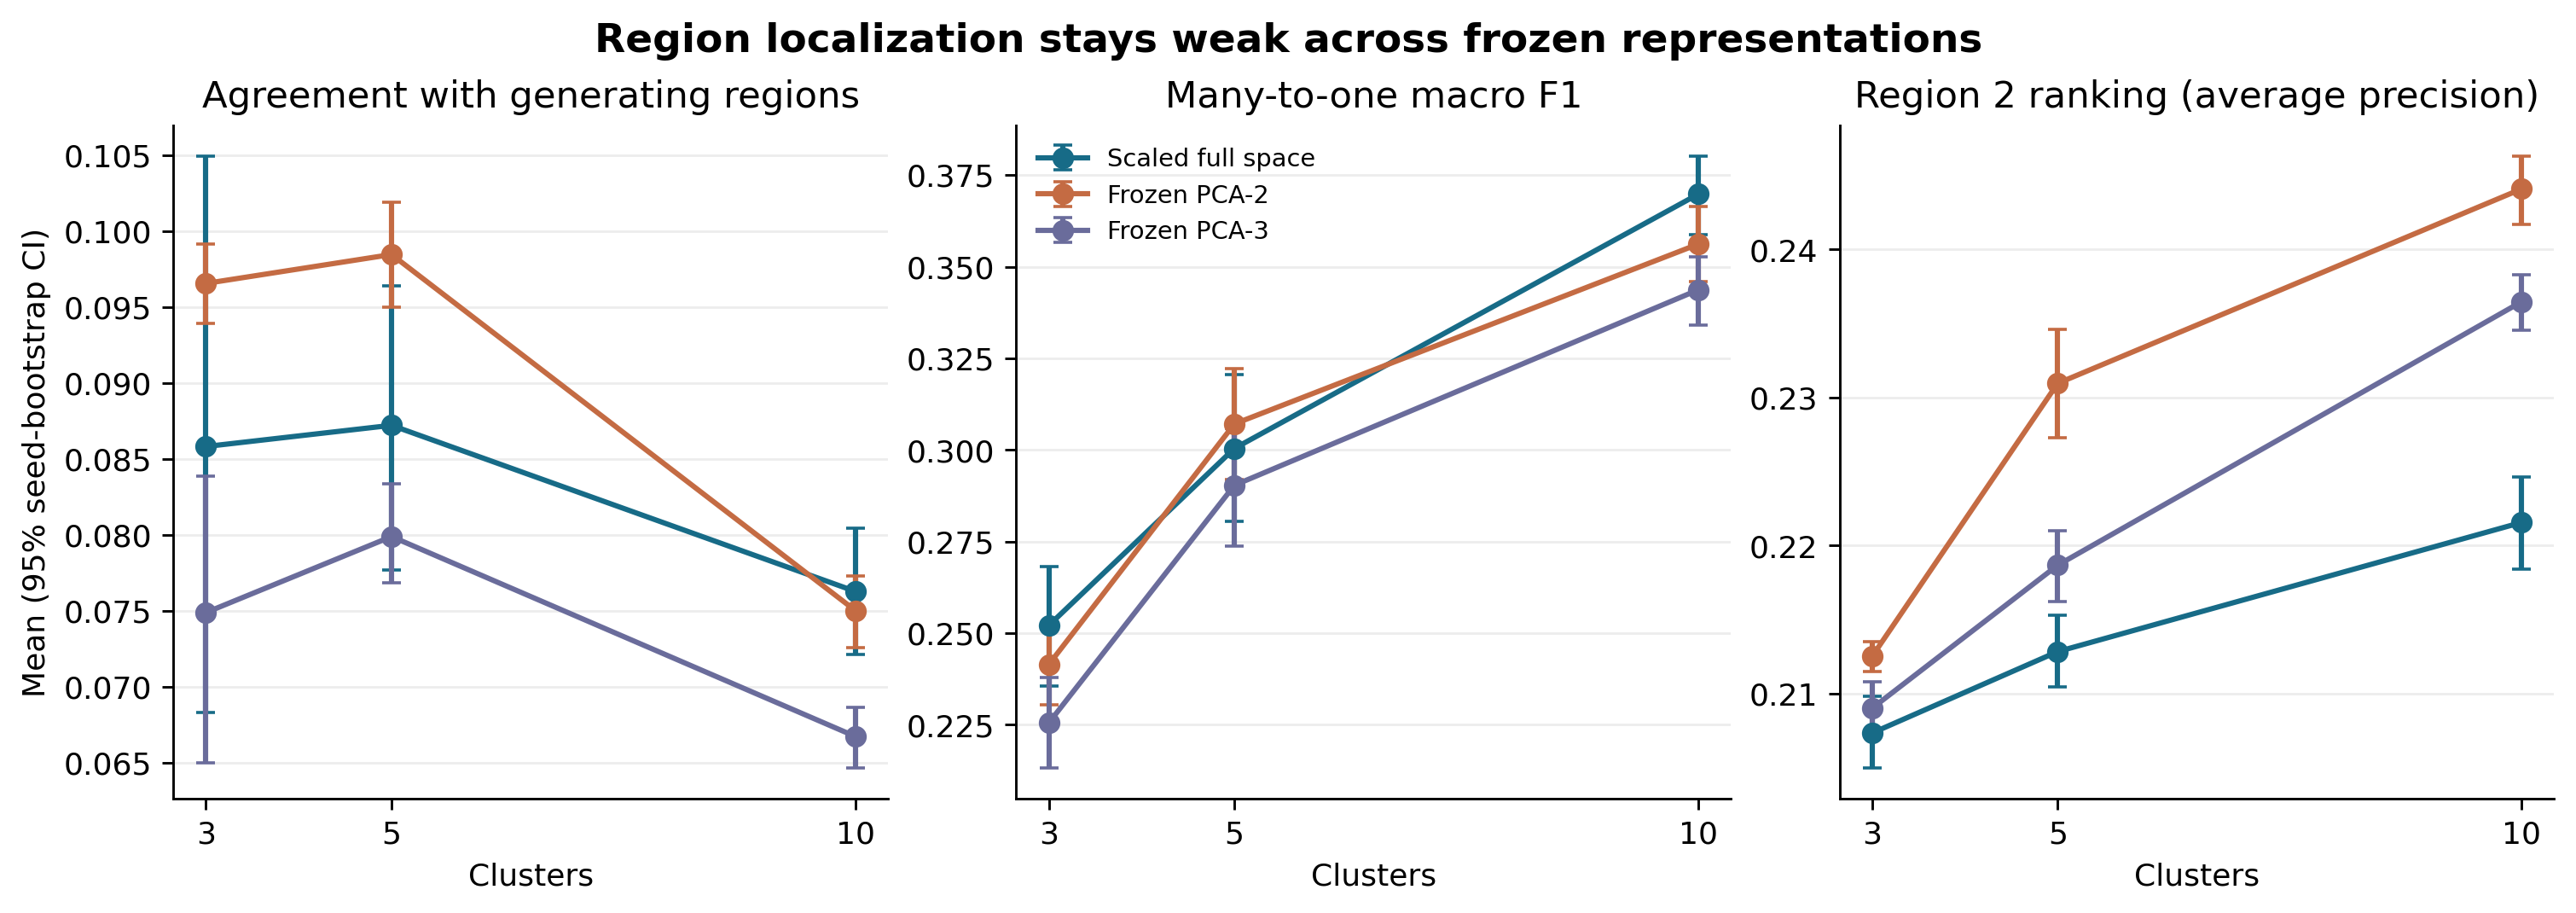
\includegraphics[width=\linewidth]{cluster_mapping_sensitivity.png}\end{center}
\section*{Limits and implication}
This sensitivity analysis does not establish a general localization method, causal attribution, or natural-stream regional validity. Region 2 has approximately one-fifth prevalence, so average precision must be read against that baseline. The results are exploratory, use one designed five-region generator, and do not justify retuning the primary method. Cluster assignments remain descriptive summaries. Raw seed-level metrics, historical contingency tables, probability maps, environment details, and SHA-256 receipts accompany this report.
\end{document}
